% Generated from manuscript.py by build_report.py. UTF-8; compile with XeLaTeX.
\documentclass[UTF8,fontset=fandol,a4paper,11pt]{ctexart}
\usepackage[margin=23mm,top=22mm,bottom=22mm]{geometry}
\usepackage{amsmath,amssymb,graphicx,booktabs,tabularx,array,float,adjustbox}
\usepackage[font=small,labelfont=bf]{caption}
\usepackage{xcolor}
\usepackage[hidelinks,unicode]{hyperref}
\usepackage{microtype}
\usepackage{setspace}
\usepackage[section]{placeins}
\usepackage{flafter}
\captionsetup{labelsep=space}
\setstretch{1.18}
\setlength{\parskip}{3pt}
\setlength{\emergencystretch}{3em}
\setlength{\textfloatsep}{12pt}
\raggedbottom
\pagestyle{plain}
\ctexset{section={format=\Large\bfseries},subsection={format=\large\bfseries}}
\hypersetup{pdftitle={IMDB 情感分类项目报告},pdfauthor={王凯平},pdfsubject={分类性能、概率校准与融合稳定性分析},pdfkeywords={IMDB, Laya, DeBERTa-v3, 情感分类, 概率融合}}
\newcolumntype{Y}{>{\raggedright\arraybackslash}X}
\begin{document}
\begin{center}
{\LARGE\bfseries 基于多视图 Laya 与 DeBERTa-v3 异构概率融合的 IMDB 电影评论情感分类}\par
\vspace{7pt}
{\normalsize 分类性能、概率校准与融合稳定性分析}\par
\vspace{5pt}
{\small 2026 年 10 月}\par
\vspace{5pt}
{\small 姓名：王凯平\qquad 学号：240165201043}\par
{\small 班级：软件工程鲲鹏二班}\par
{\small 项目源码：\url{https://github.com/lliooly/laya-imdb}}
\end{center}
\vspace{4pt}

\section*{摘要}
% Evidence: final;supplement;suppweights;supprobust
本文研究 IMDB 电影评论二分类，构建多视图 Laya 与 DeBERTa-v3-large 的异构概率融合系统。官方训练数据划分为梯度训练、校准和开发三个子集；Laya 分支对两个微调模型分别进行温度缩放，计算前缀视图与首尾视图的概率（超长评论取两者平均），按校准系数做内部融合，再与温度校准后的 DeBERTa 正类概率等权平均。最终融合在完整 25,000 条官方测试上正确分类 24,257 条，Accuracy 为 97.028\%，Macro-F1 为 0.970280，NLL 为 0.092618，ECE 为 0.650\%；相对 Laya 双模型，准确率提高 0.684 个百分点（净多正确 171 条）。相对 DeBERTa，最终融合的准确率数值上高 0.096 个百分点，并在多项概率指标上表现更好。三组完整重训中，等权融合在两组各多正确 2 条（+0.08 个百分点），三组平均 Accuracy 与 DeBERTa 持平，均为 97.08\%，平均 ECE 从 1.328\% 降至 0.741\%。保守权重与校准权重探索在开发集上呈现小幅分类增益；重复五折交叉验证中，保守组合保持 DeBERTa 的准确率并降低 NLL，分类增益仍需独立数据确认。结果显示，异构融合在部分配置中带来小幅分类提升，并在本次实验中改善概率质量；准确率收益随模型组合和权重设置变化，为按场景选择融合策略提供了依据。数据集经过多轮使用且测试中存在重复文本，相关结果可在后续独立数据上进一步检验。

关键词：电影评论；情感分类；Laya；DeBERTa-v3；概率融合；温度校准

\section{引言}
电影评论情感分类要判断作者对整部电影的态度，局部褒贬词未必与最终立场一致。作者可能先介绍剧情，再在结尾表态；也可能认可演员却否定电影，或用挖苦表达不满。只依赖词频和局部片段，容易遗漏评价对象及语用关系。本文因此同时考察分类准确率、长文本信息保留与模型置信度。

% Evidence: audit;final
IMDB 官方训练集和测试集各有 25,000 条带标签评论，正负类各占一半\cite{maas}。训练分区内留出开发集与校准集，官方测试分区完整保留。实验保存训练配置、模型版本标识和逐样本预测，便于核对各方案的评估结果。

% Evidence: locks;comparison
ModernBERT 的编码器设计兼顾计算效率与较长上下文\cite{modernbert}。Laya 将待分类文本与类型化问题一起编码\cite{laya}；本文使用的英语模型以 ModernBERT-large 为编码器，软件版本为 laya 0.4.1，模型 revision 为 7b928d828b7b0e022f929d9bd2e44165aa270148。DeBERTa-v3 采用替换词检测和梯度解耦的嵌入共享预训练\cite{deberta}，在表示、分词与训练路径上均与 Laya 不同，可作为互补分支。结构差异是否带来收益，仍须在相同样本上比较两者的预测差异。

% Evidence: fusion;heads;robust;context;supplement;suppcost;cpufull
本文给出双视图输入、Laya 内部融合与跨模型融合的计算方法，并通过完整测试预测、配对错误变化和概率指标评价组合效果。三组完整重训与校准权重探索进一步考察融合的互补性与稳定性；决策头、损失函数与上下文长度的对照回答组件是否有效，跨后端核验回答数值是否一致，同平台 GPU 测速回答计算代价。研究重点是已有模型在本任务上的适配、组合，以及可复核的效果分析。

\section{数据集与实验协议}
\subsection{数据清洗与固定划分}
% Evidence: audit
数据来自 Stanford 发布的 Large Movie Review Dataset\cite{maas}。预处理包括：将 HTML 换行标记替换为空格、还原 HTML 实体、压缩连续空白；保留大小写与标点，不使用停用词删除或词干化，以保留否定、程度及反讽线索。训练集与开发集按清洗文本分组后进行分层划分，划分策略规定，同一文本出现冲突标签的组只保留在训练侧。审计结果显示，训练集与开发集唯一的清洗文本交集为 0。

% Evidence: audit;deberta;final
\begin{table}[htbp]\centering\caption{固定数据分区及用途}\label{tab:t1}\small\renewcommand{\arraystretch}{1.25}
\begin{tabularx}{\linewidth}{YYY}\toprule
\textbf{分区} & \textbf{样本数} & \textbf{用途}\\\midrule
梯度训练 & 22,100 & 模型参数更新\\
校准 & 400 & 温度、既定权重或拒答阈值\\
开发 & 2,500 & 方案比较与诊断\\
官方测试 & 25,000 & 冻结方案的完整评分\\
\bottomrule\end{tabularx}\end{table}
% Evidence: audit;deberta;final;reviewaudit
原始官方训练集先按 seed 42 划分为 22,500 条训练池和 2,500 条开发集，再从训练池中按校准随机种子 42 留出 400 条，得到 22,100 条梯度训练样本。开发集每类 1,250 条；校准集包含 185 条负类和 215 条正类。原始官方训练集与测试集之间有 123 条唯一清洗文本重叠，其中落在实际梯度训练集的有 113 条（对应 113 条测试样本）。完整官方测试评分保留这些样本，其独立性限制见第 6.2 节。

% Evidence: audit;oldtest
\begin{figure}[htbp]\centering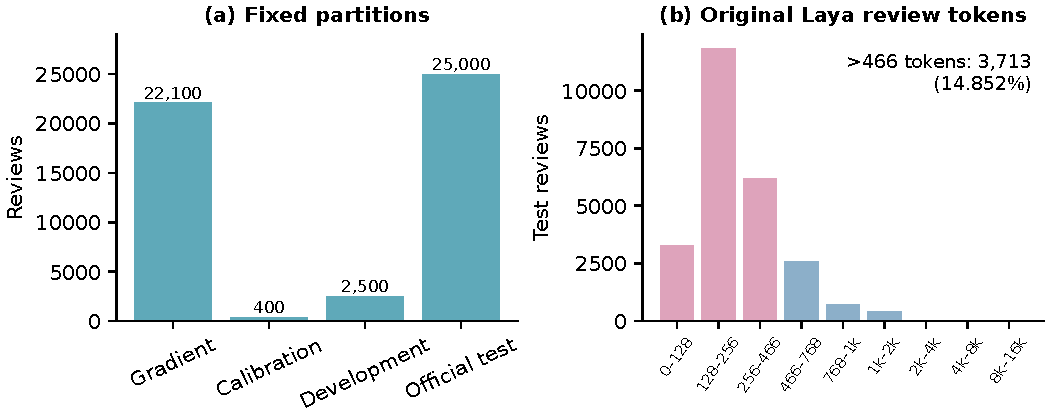
\includegraphics[width=\linewidth]{figures/02_data.pdf}\caption{数据规模与官方测试评论长度。右图长度来自保存的原 Laya 分词统计，横轴为离散长度区间；长度不代表 DeBERTa 的分词长度。官方测试有 3,713 条超过 Laya 的 466 token 评论预算，占 14.852\%。}\label{fig:f1}\end{figure}
\subsection{训练、校准与评估的边界}
% Evidence: final;fusion;deberta
梯度训练集用于模型参数更新；400 条校准集用于温度、融合系数和拒答阈值的估计；开发集用于方案比较。最终官方测试前冻结模型版本、输入策略、温度、融合规则和执行后端。评估时按唯一样本 ID 对齐输入、标签与概率。

% Evidence: comparison;heads
本文不把训练预算不同的历史模型之间的分数差解释为某一机制的因果效应。例如 ModernBERT-base 历史结果采用 256 token，Laya 采用更大的编码器与 512 token 总预算，两者可作方案比较，但不能单独证明类型化决策头有效。后续决策头实验采用共同的 Laya 编码器并重新初始化决策头，其结论也只适用于该预训练编码器与该训练预算。

\section{模型与方法}
\subsection{Laya 类型化情感决策}
% Evidence: comparison;traincode
Laya 把评论文本作为待分类状态（state），问题类型设为选择式（choice）。实际英文问题为“What is the reviewer's overall opinion of this movie?”；negative 的判定标准为“The reviewer dislikes or criticizes the movie overall.”，positive 为“The reviewer likes or praises the movie overall.”。训练时随机置换候选顺序，评分时再按候选语义把分数对应回负类与正类。模型采用两层 Transformer 决策头与候选 [MASK] 位置评分结构\cite{laya}。式~\eqref{eq:e1}中 m 表示 Laya 模型，v 表示输入视图，z\_c 表示候选 c 的分数；编码器记为 E\_m，类型化问题模板记为 q，决策头记为 H\_m，类别分数如下。

\begin{equation}\label{eq:e1}\begin{adjustbox}{max width=.94\linewidth}$\displaystyle \mathbf z_{m,v}(x)=H_m\!\left(E_m\left(\operatorname{pack}(v(x),q)\right)\right),\qquad \hat y=\arg\max_{c\in\{0,1\}}z_c.$\end{adjustbox}\end{equation}
% Evidence: comparison;combinedconfig
模型主要采用监督交叉熵（cross-entropy，CE）训练。对单条样本，类别目标为 y，预测概率为 p；当目标分布为 one-hot 时，式~\eqref{eq:e2}即退化为普通交叉熵。部分组合配方使用 0.05 标签平滑，另有校准决策强化学习（Reinforcement Learning for Calibrated Decisions，RLCD）先导实验\cite{laya}。该先导实验与全数据 CE 训练使用不同的样本预算，因此两者的差值不能作为单独改变损失函数的消融结果。

\begin{equation}\label{eq:e2}\begin{adjustbox}{max width=.94\linewidth}$\displaystyle \mathcal L_{\rm CE}=-\sum_{c=0}^{1}\widetilde y_c\log p_c,\qquad \widetilde y_c=(1-\varepsilon)\,\mathbb 1[y=c]+\varepsilon/2.$\end{adjustbox}\end{equation}
\subsection{长度约束与双视图概率}
% Evidence: fusion;oldtest
主方案将 Laya 的输入总长度上限设为 512 token，决策头输入长度上限设为 192 token；问题与候选模板及分隔符占去 46 token 后，评论可用 466 token。两个 Laya 模型训练时均采用前缀输入；推理时增加首尾视图，对超长评论保留原分词序列的首 233 与末 233 token。对不超过评论预算的样本，两种视图的输入相同，复用同一次前向；超长样本再计算首尾视图。式~\eqref{eq:e3}中 m 表示 Laya 模型，\ensuremath{\ell}\_m 表示该模型分词器下的原评论长度。

\begin{equation}\label{eq:e3}\begin{adjustbox}{max width=.94\linewidth}$\displaystyle \bar p_m(x)=\begin{cases}p_{m,\mathrm{prefix}}(x),& \ell_m(x)\le466,\\[2pt]\frac12\left[p_{m,\mathrm{prefix}}(x)+p_{m,\mathrm{headtail}}(x)\right],&\ell_m(x)>466.\end{cases}$\end{adjustbox}\end{equation}
% Evidence: fusion;deberta
式~\eqref{eq:e4}中的 p 为正类概率。baseline-s43 与 combined-s42 分别沿用训练阶段在 400 条校准样本上得到的温度 1.7130507231 和 0.9167026281；DeBERTa 的温度为 1.1374971946，由相同校准集上的 NLL 最小化得到。融合阶段沿用这些温度。温度缩放把 logits 统一除以正温度 T，再计算 softmax\cite{guo}；它不改变模型单次前向输出的类别排序，只改变融合时使用的概率尺度。

\begin{equation}\label{eq:e4}\begin{adjustbox}{max width=.94\linewidth}$\displaystyle p_{m,v}(y=1\mid x)=\operatorname{softmax}\!\left(\mathbf z_{m,v}(x)/T_m\right)_1.$\end{adjustbox}\end{equation}
\subsection{Laya 内部融合与 DeBERTa 异构分支}
% Evidence: fusion;combinedconfig;baseconfig
Laya 分支使用 baseline-s43 与 combined-s42：前者为 seed 43 的基线配方，后者为 seed 42 的预热（warmup）与标签平滑组合配方。内部融合系数 \ensuremath{\lambda} 在 400 条校准样本上通过最小化 NLL + 0.01(\ensuremath{\lambda}−0.5)² 求得，约束在 [0,1] 内，结果为 \ensuremath{\lambda}=0.7020326698。最终系统包含这两个 Laya checkpoint 和一个 DeBERTa checkpoint。

\begin{equation}\label{eq:e5}\begin{adjustbox}{max width=.94\linewidth}$\displaystyle p_{\rm Laya}(x)=\lambda\bar p_{\rm baseline\text{-}s43}(x)+(1-\lambda)\bar p_{\rm combined\text{-}s42}(x).$\end{adjustbox}\end{equation}
% Evidence: deberta;debertaconfig;final;debertacode;cpufull
DeBERTa-v3-large 使用独立的 SentencePiece 分词器。512 token 总预算中有 2 个特殊 token，评论预算为 510 token；超长评论保留首 255 与末 255 token。原固定分支以 seed 42 训练两轮，开发推理采用 CUDA BF16，最终测试采用本地 CPU FP32；Laya 测试分支复用已保存的 CUDA FP32 概率。后端切换的准入检查中，400 条校准与 128 条开发样本的预测类别均一致。补充核验进一步覆盖相同旧权重与温度下的全部 2,500 条开发样本：DeBERTa 类别变化 1 条，最终融合类别变化 0 条，最大概率绝对差为 0.011909。这说明在全部开发样本上融合分类保持一致；不同精度下的概率不保证逐位相同。

\begin{equation}\label{eq:e6}\begin{adjustbox}{max width=.94\linewidth}$\displaystyle p_{\rm final}(x)=\tfrac12p_{\rm Laya}(x)+\tfrac12p_{\rm DeBERTa}(x),\qquad \hat y=\mathbb 1[p_{\rm final}(x)\ge0.5].$\end{adjustbox}\end{equation}
% Evidence: weight
式~\eqref{eq:e6}中的融合比例在测试前固定为 50:50。另一个仅最小化校准 NLL 的单系数对照得到 Laya 21.94\%、DeBERTa 78.06\% 的权重。开发集上 NLL 从 0.088768 降至 0.088108，准确率从 97.28\% 变为 97.16\%：修复 8 条、退化 11 条，净少正确 3 条，精确 McNemar p=0.6476。这说明降低 NLL 与提高分类正确数并不是同一个优化目标。

% Evidence: fusion;deberta;final
\begin{figure}[htbp]\centering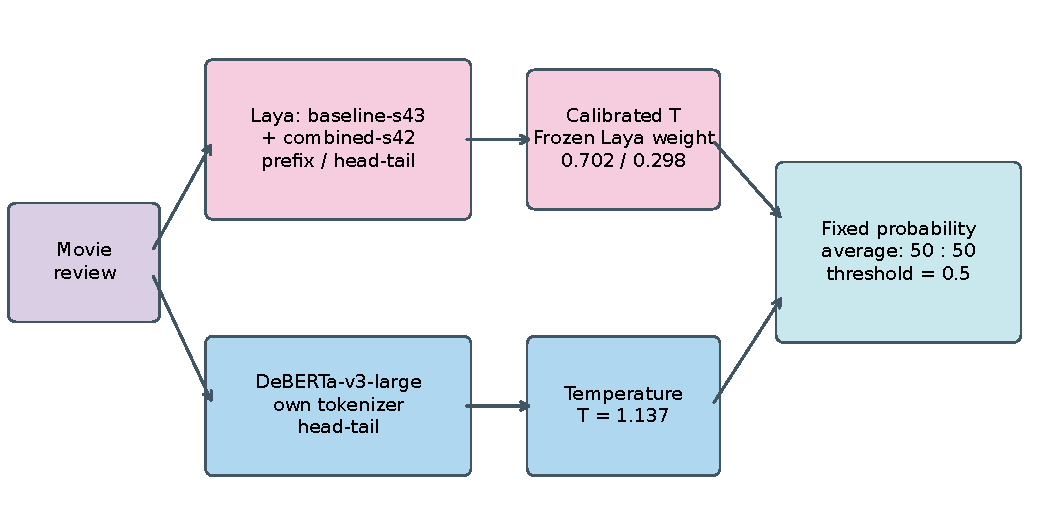
\includegraphics[width=\linewidth]{figures/01_pipeline.pdf}\caption{最终冻结方案的计算流程示意。Laya 分支包含两个模型，DeBERTa 分支包含一个模型；两分支在各自校准后等权融合。该图仅示意方法流程，不代表实验结果。}\label{fig:f2}\end{figure}
% Evidence: architecture;archfacts;locks;debertalock
图~\ref{fig:f3} 进一步展开模型内部结构。每个 Laya checkpoint 使用 28 层 ModernBERT-large 编码器，并在各 token 的输出上加入 choice 类型嵌入；随后经过两层前置 LayerNorm 的 Transformer 决策块，最后提取两个候选 [MASK] 位置，由共享评分网络分别得到负类与正类 logits。DeBERTa-v3-large 使用 24 层编码器，经首 token 池化与线性分类头输出两类 logits。图中层叠方块表示共同结构，baseline-s43 与 combined-s42 的参数仍彼此独立。右侧放大图保留自注意力与前馈子层的残差连接；上游 action head 不参与本次情感概率融合，因此未在图中画出。

% Evidence: architecture;archfacts;locks;debertalock
\begin{figure}[htbp]\centering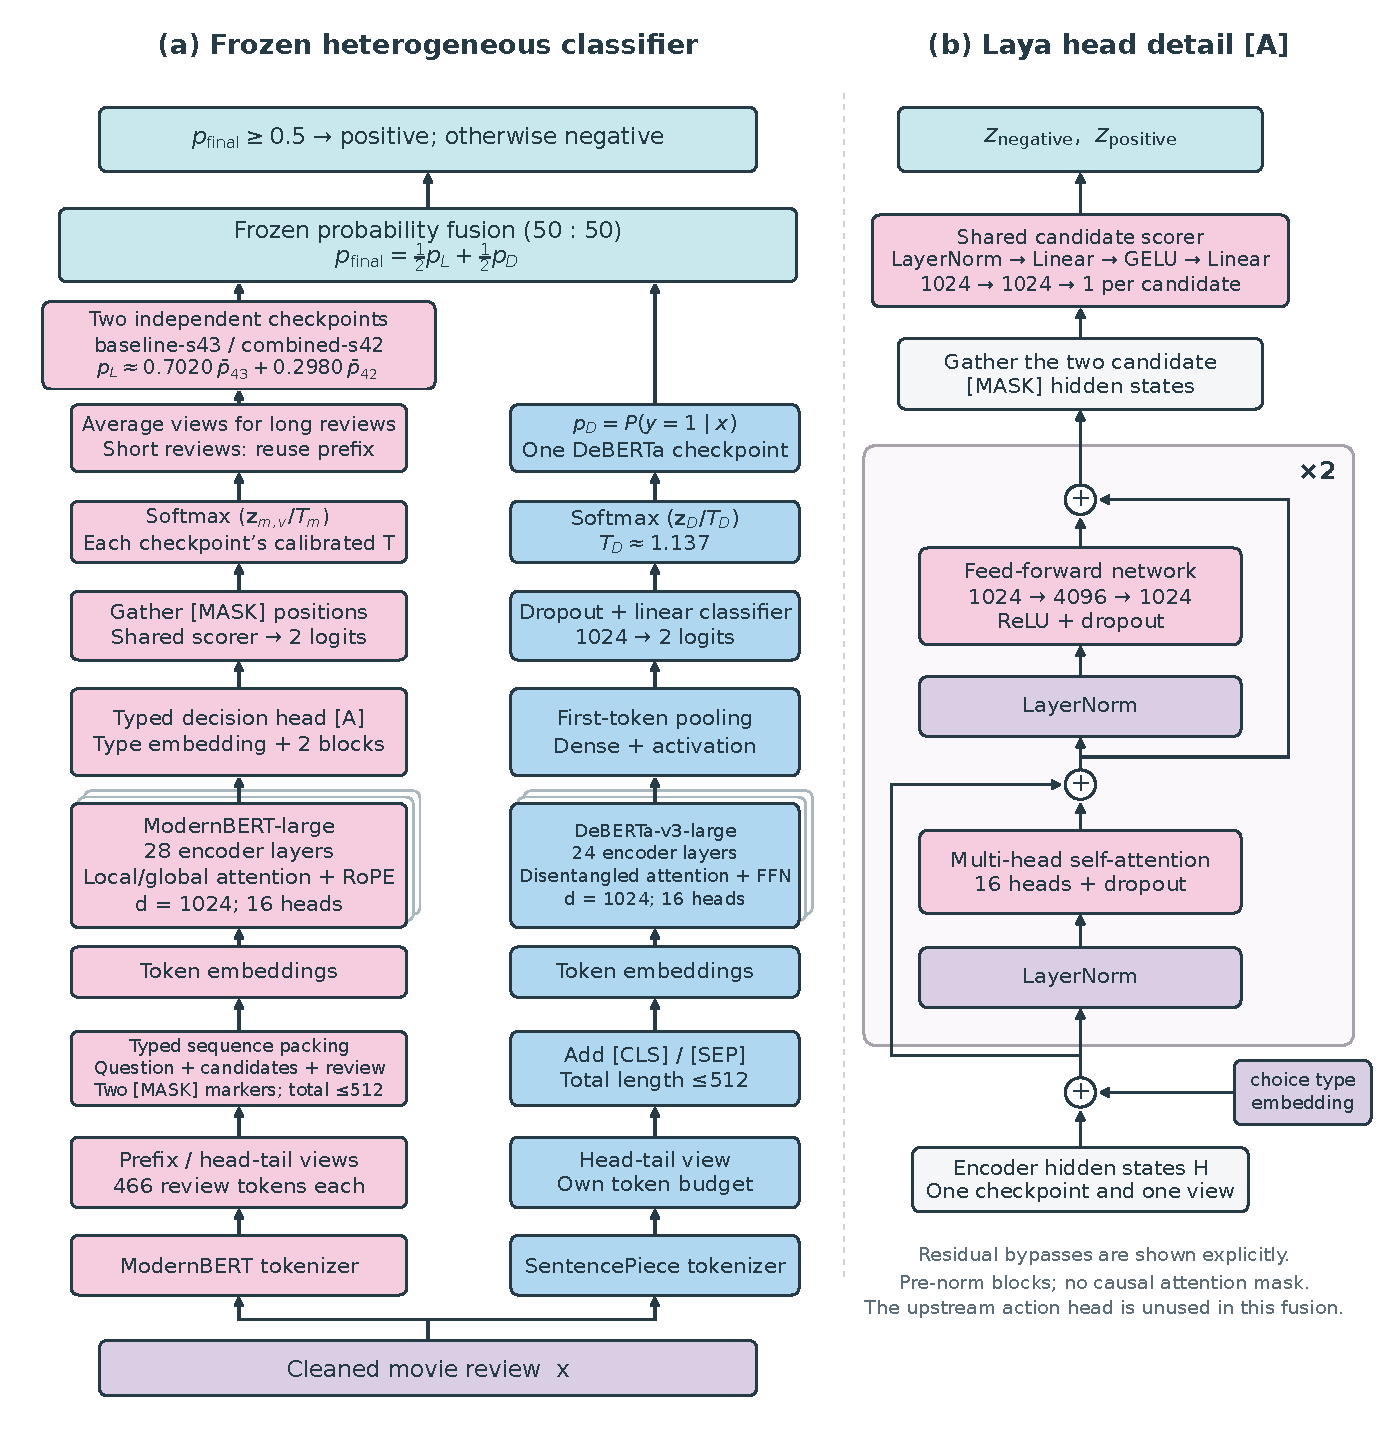
\includegraphics[width=\linewidth]{figures/11_architecture.pdf}\caption{最终模型架构与 Laya 决策头局部放大。数据流自下而上：左侧为多视图 Laya、DeBERTa 与冻结的概率融合，右侧展开标记 [A] 的决策头。堆栈标明编码器层数，×2 表示两个前置 LayerNorm 决策块；两个 Laya checkpoint 使用独立权重。本图按冻结配置和实际源码绘制，未包含新的实验内容。}\label{fig:f3}\end{figure}
\section{实验设置与评价指标}
\subsection{训练配置与运行平台}
% Evidence: baseconfig;combinedconfig;debertaconfig
\begin{table}[htbp]\centering\caption{构成最终方案的训练配方摘要}\label{tab:t2}\small\renewcommand{\arraystretch}{1.25}
\begin{tabularx}{\linewidth}{YYY}\toprule
\textbf{项目} & \textbf{Laya 两个既有模型} & \textbf{DeBERTa-v3-large}\\\midrule
训练轮数 / seed & 2 轮；43 / 42 & 2 轮；42\\
最大总长度 & 512；评论预算 466 & 512；扣除自身特殊 token\\
micro-batch / 累积 & 8 / 1 & 8 / 4\\
初始学习率 & 编码器 2.5e−5；头 1e−4 & 1e−5\\
weight decay / clip & 0.01 / 1.0 & 0.01 / 1.0\\
调度 & 余弦；组合配方 5\% 预热 & 线性；83 步预热 / 1,382 总更新\\
平滑系数 & baseline 0；combined 0.05 & 普通监督分类\\
训练计算精度 & CUDA FP32；AMP 关闭 & CUDA BF16；FP32 主参数\\
\bottomrule\end{tabularx}\end{table}
% Evidence: comparison;regularization;robust;mlx
研究在 Apple M5 Pro（MPS/MLX 后端）、本地 CPU 与 CUDA GPU 三种环境上进行。历史正则化实验使用 RTX 4090；部分决策头、损失和后续训练使用单独锁定的云端环境。各阶段的设备、依赖、精度与计时口径不同，本文只对同协议的测量作直接比较，不把不同硬件、不同阶段的耗时合并成统一的效率比较。

\subsection{分类、概率与不确定性指标}
% Evidence: final;analysiscode
主指标为全覆盖准确率（Accuracy），并报告宏平均 F1（Macro-F1）与受试者工作特征曲线下面积（area under the ROC curve，AUROC）。概率质量用负对数似然（negative log-likelihood，NLL）、正类 Brier score 与期望校准误差（expected calibration error，ECE）衡量。ECE 使用 15 个等宽置信分箱，按 top-label 口径计算，表中以百分数表示；二分类置信度为 max(p,1−p)，空箱不计入 ECE。AUROC 衡量排序质量，不能替代 Accuracy 或校准误差。

\begin{equation}\label{eq:e7}\begin{adjustbox}{max width=.94\linewidth}$\displaystyle \operatorname{NLL}=-\frac1n\sum_{i=1}^{n}\left[y_i\log p_i+(1-y_i)\log(1-p_i)\right],\qquad \operatorname{Brier}_{+}=\frac1n\sum_i(p_i-y_i)^2.$\end{adjustbox}\end{equation}
\begin{equation}\label{eq:e8}\begin{adjustbox}{max width=.94\linewidth}$\displaystyle \operatorname{ECE}=\sum_{b=1}^{15}\frac{|B_b|}{n}\left|\operatorname{acc}(B_b)-\operatorname{conf}(B_b)\right|.$\end{adjustbox}\end{equation}
% Evidence: final;heads;robust
单方案 Accuracy 报告 Wilson 95\% 区间。同一批 ID 上的固定方案采用精确双侧 McNemar 检验，并报告修复数、退化数与按类别分层的配对 bootstrap 百分位区间。最终测试使用 20,000 次重采样、随机种子 20261018；三个随机种子的决策头与损失对照各使用 10,000 次重采样、随机种子 20261015；同一次重采样中，各模型使用相同的样本，从而保持配对关系。这些区间在模型与校准参数固定的条件下计算，只描述样本层面的不确定性。历史模型的六组比较与后续融合的四候选比较分别采用 Holm 校正，后者调整后 p 值均为 1；整个研究未做跨实验的多重比较校正。

\section{实验结果与分析}
\subsection{开发集与完整官方测试}
% Evidence: deberta;final
\begin{table}[H]\centering\caption{固定主方案的开发与官方测试结果（DeBERTa 开发集使用 CUDA BF16，测试集使用 CPU FP32）}\label{tab:t3}\small\renewcommand{\arraystretch}{1.25}
\footnotesize\setlength{\tabcolsep}{3pt}
\begin{tabular*}{\linewidth}{@{\extracolsep{\fill}}l l r r r r r@{}}\toprule
\textbf{数据} & \textbf{方案} & \textbf{正确 / 总数} & \textbf{Accuracy} & \textbf{Macro-F1} & \textbf{NLL} & \textbf{ECE}\\\midrule
开发 & Laya 双模型 & 2,424 / 2,500 & 96.960\% & 0.969599 & 0.106593 & 1.292\%\\
开发 & DeBERTa BF16 & 2,426 / 2,500 & 97.040\% & 0.970400 & 0.093473 & 1.326\%\\
开发 & 最终融合 & 2,432 / 2,500 & 97.280\% & 0.972800 & 0.088768 & 0.916\%\\
测试 & Laya 双模型 & 24,086 / 25,000 & 96.344\% & 0.963440 & 0.114159 & 1.204\%\\
测试 & DeBERTa FP32 & 24,233 / 25,000 & 96.932\% & 0.969319 & 0.095947 & 1.363\%\\
测试 & 最终融合 & 24,257 / 25,000 & 97.028\% & 0.970280 & 0.092618 & 0.650\%\\
\bottomrule\end{tabular*}\end{table}
% Evidence: final
如表~\ref{tab:t3} 和图~\ref{fig:f4} 所示，最终融合的完整官方测试 Accuracy 为 97.028\%，Wilson 95\% 区间为 [96.810\%, 97.231\%]；Macro-F1 为 0.970280，AUROC 为 0.994350。Laya 双模型的 AUROC 为 0.992436，DeBERTa 为 0.994449。最终融合在分类正确数与多项概率指标上均有提升；排序性能与 DeBERTa 接近而略低，说明不同指标之间存在取舍。

% Evidence: deberta;final
\begin{figure}[htbp]\centering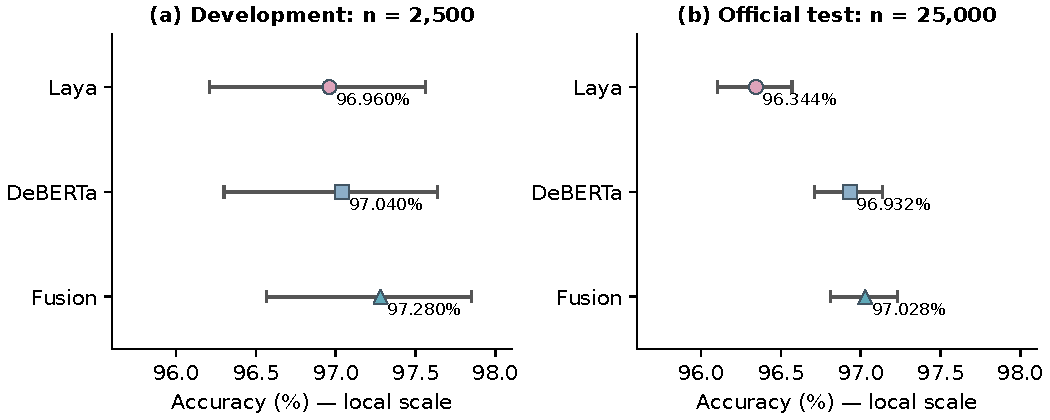
\includegraphics[width=\linewidth]{figures/03_accuracy.pdf}\caption{固定模型的准确率与 Wilson 95\% 区间。横轴为截断尺度（局部放大，已在图上标出）；开发与测试分开显示。误差线不包含训练或模型选择不确定性，也不用于单独判断配对差异。}\label{fig:f4}\end{figure}
% Evidence: alternatives;bow
开发集上的正则化 logit 探索达到 97.40\%，相对冻结的 97.28\% 方案净多正确 3 条，名义 McNemar p=0.25，四候选 Holm 校正后 p=1；其 NLL 与 ECE 未同步改善，也没有对应的完整官方测试结果。TF-IDF 分支融合达到 97.32\%（净增 1 条），NB-ngram 融合为 97.28\%。这些探索覆盖了多个方向，但最终方案仍按测试前冻结的规则确定。词袋分支借鉴 NB 加权 n-gram 思路\cite{wang}，并不是对原论文所有模型的精确复现。

\subsection{配对错误变化与收益来源}
% Evidence: final
相对 Laya 双模型，最终融合修复 265 条错误，同时使原本正确的 94 条变成错误，净变化为 +171 条；Accuracy 增加 0.684 个百分点，条件配对 bootstrap 95\% 区间为 [+0.536, +0.832] 个百分点，精确 McNemar p=5.538\ensuremath{\times10^{-20}}。此前的 Laya 双模型错误数为 914 条，最终融合为 743 条，相对错误减少率为 171/914\ensuremath{\approx}18.71\%。相对此前的 Laya 双模型，最终融合的改进在实测中成立。

% Evidence: analysiscode;final
相对 DeBERTa 单分支，最终融合修复 144 条、退化 120 条，净多正确 24 条，即 +0.096 个百分点；在冻结概率上独立复算，精确 McNemar 检验给出 p=0.1568。引入 DeBERTa 之后相对 Laya 双模型的改进，与“融合是否稳定优于最强单分支”，是两个不同的问题；前者检验的是相对 Laya 系统的改进，后者检验的是相对最强单分支的增量，两者不能混用。后者的证据目前以观察性为主，可通过更多训练重复进一步加强。

% Evidence: final
\begin{figure}[htbp]\centering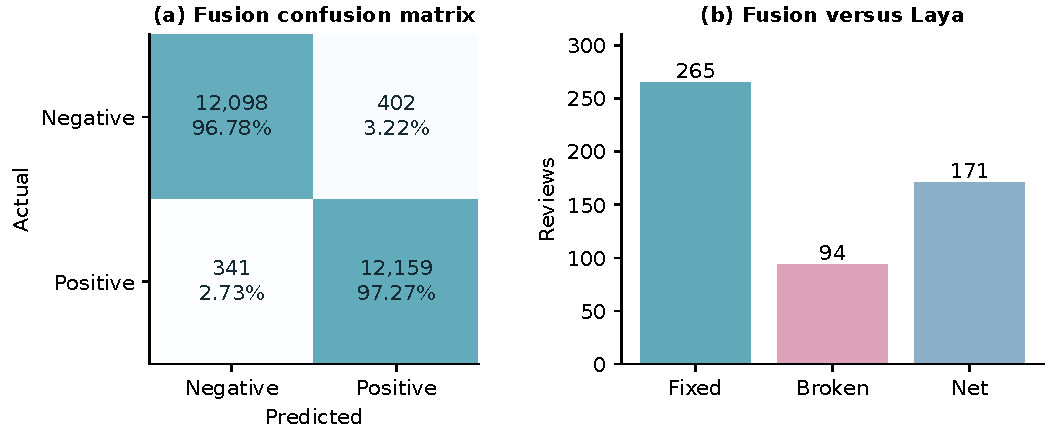
\includegraphics[width=\linewidth]{figures/04_errors.pdf}\caption{左：最终融合的官方测试混淆矩阵，行为真实标签、列为预测标签，每行分母为 12,500。右：相对 Laya 双模型的样本级修复、退化与净增量；修复与退化都列出，以免只呈现修复的一面。}\label{fig:f5}\end{figure}
% Evidence: final
最终混淆矩阵的四个元素为：负类判对 12,098、负类判成正类 402、正类判成负类 341、正类判对 12,159。两类召回分别为 96.784\% 与 97.272\%，相差 0.488 个百分点。类别平衡使 Accuracy 与 Macro-F1 接近；具体方向的错误仍值得关注，而混淆矩阵本身不能解释模型内部为何误判。

\subsection{概率校准和置信度}
% Evidence: final
完整测试上，最终融合的 NLL 为 0.092618，低于 Laya 双模型的 0.114159 和 DeBERTa 的 0.095947；ECE 为 0.650\%，也低于两分支的 1.204\% 和 1.363\%。正类 Brier score 依次为：最终融合 0.024172、DeBERTa 0.025002、Laya 双模型 0.029499。图~\ref{fig:f6} 同时展示这三项指标，避免只依据一种分箱统计判断校准效果。

% Evidence: final
\begin{figure}[htbp]\centering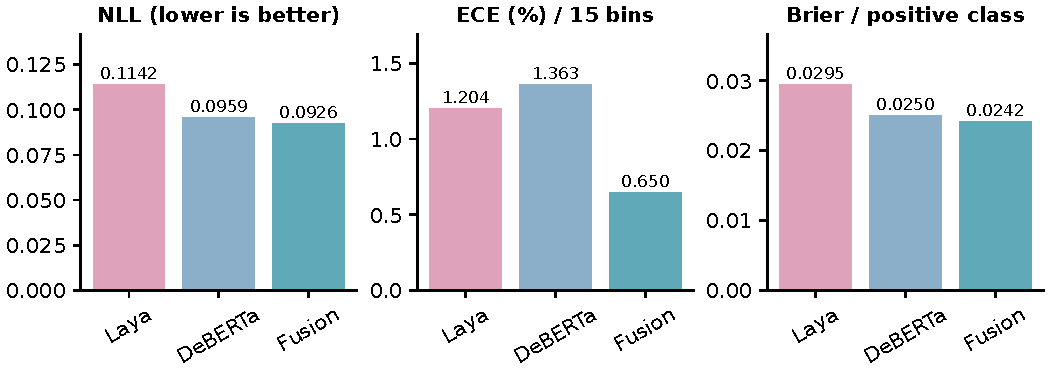
\includegraphics[width=\linewidth]{figures/05_probability.pdf}\caption{完整官方测试的三项概率指标。条形图坐标轴从零开始；NLL、ECE 与 Brier 越低越好。ECE 是有限样本、依赖分箱方式的描述量，不能保证单条预测的概率。}\label{fig:f6}\end{figure}
% Evidence: final
\begin{figure}[htbp]\centering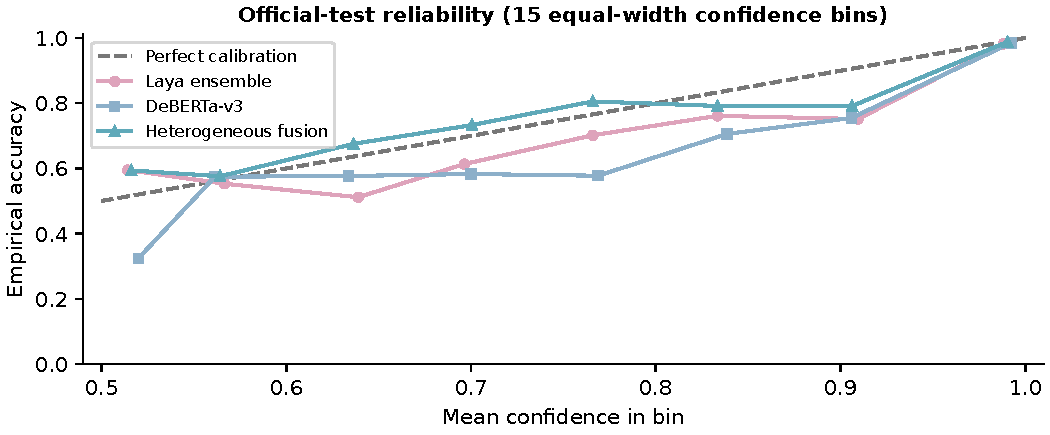
\includegraphics[width=\linewidth]{figures/06_reliability.pdf}\caption{官方测试可靠性曲线。沿用原始 15 等宽置信分箱，只绘制非空箱；低置信箱样本较少，局部折线波动不能直接解释为稳定规律。每箱分母与数值保存在 analysis/reliability\_bins.csv。}\label{fig:f7}\end{figure}
% Evidence: final;devanalysis
将置信度不低于 0.95 的误分类样本定义为高置信度错误，其比例以全部错误为分母。最终融合为 244/743=32.8\%，Laya 双模型为 375/914=41.0\%，DeBERTa 为 308/767=40.2\%；最终融合错误样本的平均置信度为 0.812。这些结果表明，本次冻结方案减轻了模型的过度自信。置信度排序可用于人工复核与选择性输出；全覆盖分类、固定覆盖下的排序曲线与按校准阈值部署后的实际覆盖率具有不同分母，应分别报告。

\subsection{文本长度与误差分层}
% Evidence: final
\begin{table}[htbp]\centering\caption{按原 Laya 评论预算分层的官方测试 Accuracy}\label{tab:t4}\small\renewcommand{\arraystretch}{1.25}
\begin{tabularx}{\linewidth}{YYYYY}\toprule
\textbf{分组} & \textbf{n} & \textbf{Laya 双模型} & \textbf{DeBERTa} & \textbf{最终融合}\\\midrule
\ensuremath{\le}466 token & 21,287 & 96.345\% & 96.970\% & 97.050\%\\
>466 token & 3,713 & 96.337\% & 96.714\% & 96.903\%\\
\bottomrule\end{tabularx}\end{table}
% Evidence: final
最终融合在未截断与截断两组均高于 Laya 双模型，分别净多正确 150 与 21 条。该分层仅按 Laya 分词器的 466 token 预算定义；DeBERTa 使用自己的分词器，因此不能把两组直接对应为“两个模型都读全”或“都截断”。分层差值只是描述性结果，本文未单独检验长度与模型之间的交互效应。

% Evidence: final;robust
\begin{figure}[htbp]\centering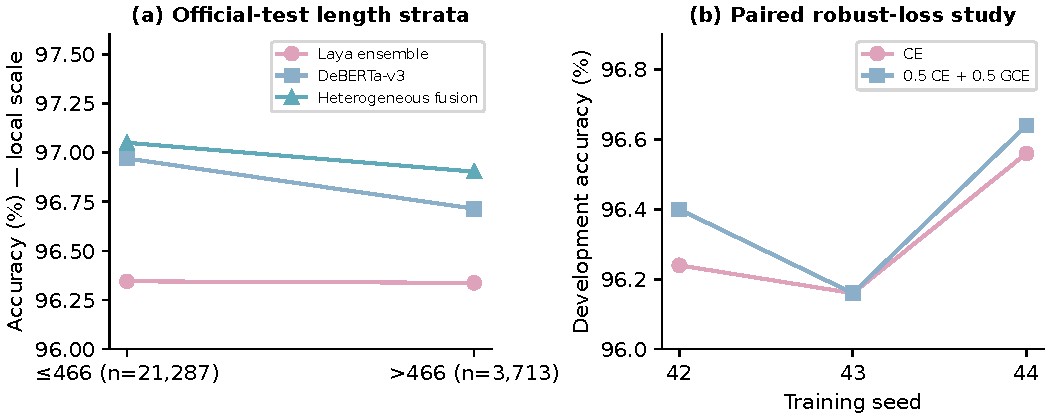
\includegraphics[width=\linewidth]{figures/07_strata_ablation.pdf}\caption{左：官方测试长度分层；右：独立的三随机种子 CE / mixed 开发对照，列出全部种子结果，而不是只挑最优种子。两个面板来自不同实验，样本范围也不同。}\label{fig:f8}\end{figure}
\subsection{受控消融与配置敏感性}
% Evidence: heads;robust;context;reviewed;weight;alternatives
\begin{table}[htbp]\centering\caption{主要受控实验与探索结果概览}\label{tab:t5}\small\renewcommand{\arraystretch}{1.25}
\begin{tabularx}{\linewidth}{YYY}\toprule
\textbf{实验} & \textbf{观察结果} & \textbf{证据解释}\\\midrule
决策头：3 seeds & 原始 96.520\%；线性 96.493\% & 均值差 +0.027 个百分点；两种头差异很小\\
鲁棒损失：3 seeds & CE 96.32\%；mixed 96.40\% & 均值差 +0.08 个百分点；条件区间跨零\\
512 → 2,048 & 总体 96.32\% → 96.32\% & 长组 +6，短组 −6\\
训练标签修订 v2 & 96.32\% → 96.40\% & 净 +2；p=0.883\\
校准拟合外层权重 & 97.28\% → 97.16\% & NLL 改善；Accuracy 数值略降\\
正则化 logit 探索 & 开发 97.40\% & 净 +3；未进行正式测试\\
\bottomrule\end{tabularx}\end{table}
% Evidence: heads
决策头对照使用相同的预训练编码器、训练输入与预算，比较重新初始化的原始头与线性头。seed 42、43、44 下，原始头减线性头的 Accuracy 差分别为 −0.20、+0.20、+0.08 个百分点，均值 +0.0267，条件 95\% 区间为 [−0.2533, +0.3067]；两种头的准确率差异很小。线性头的平均训练总耗时少 6.81\%（含模型与数据准备、两轮训练、逐轮保存及保存前校准参考前向）、峰值已分配显存少 4.94\%、可训练参数少 6.23\%；推理吞吐目前尚无独立测量。

% Evidence: robust
鲁棒损失采用 0.5 CE + 0.5 GCE(q=0.7)，其中 GCE 为广义交叉熵（generalized cross-entropy）\cite{gce}，单样本损失为 [1 − (p\_y 的 q 次幂)] / q，p\_y 为真实类别的预测概率。三个种子的 Accuracy 差为 +0.16、0.00、+0.08 个百分点，平均 +0.08，条件区间为 [−0.174, +0.347]；截断组平均低 0.328 个百分点。混合损失的收益幅度很小，且主要来自未截断样本，值得在更多种子上继续验证。

% Evidence: context
长度对照采用固定 seed 42、两轮训练与相同的样本曝光量，2,048 与 512 的总体准确率均为 96.32\%；2,048 修复 23 条并退化 23 条。截断组净增 6 条、未截断组净减 6 条，说明在该配置下，增加上下文对截断样本有正向作用、对未截断样本有负向作用，总体持平。这里的“同预算”只指训练样本数与轮数相同，不表示 token 计算量、显存占用或实际训练时间相同。

% Evidence: heads;context
\begin{figure}[htbp]\centering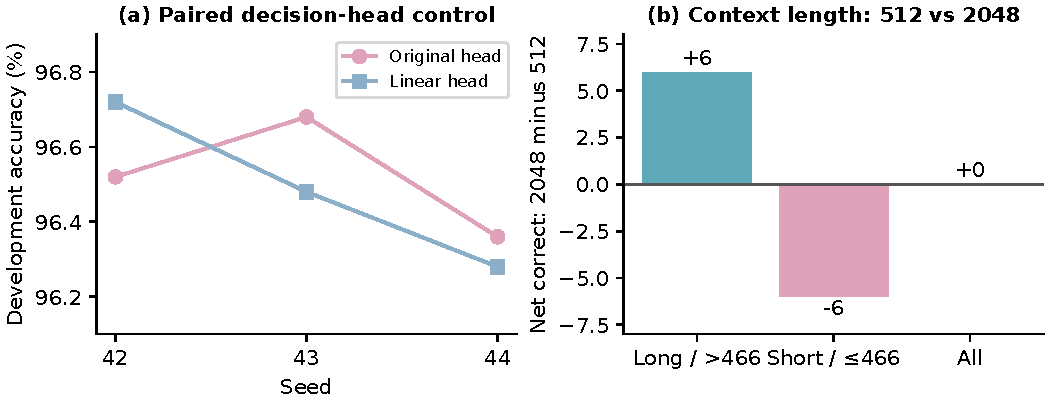
\includegraphics[width=\linewidth]{figures/08_controls.pdf}\caption{左：共同预算下原始头与线性头的全部种子结果，纵轴为截断尺度（已在图上标出）。右：独立长度对照中 2,048 相对 512 的净正确数变化；总体净变化为零。}\label{fig:f9}\end{figure}
% Evidence: reviewed
训练数据修订单独保存派生版本：94 条复核候选最终包含 61 条改标、3 条删除；原始版本及其标签、划分仍完整保留。按原开发标签评估，准确率从 96.32\% 升至 96.40\%，p=0.883。复核提高了局部语义一致性；其稳定泛化收益可在更多种子上继续验证。本文没有因开发或测试案例而改写最终评分标签。

\subsection{跨后端数值核验与工程成本}
% Evidence: mlx
跨后端评估同时比较 logits、概率与类别。此前的 MLX FP16 候选有 1 条概率差超过 0.01 的预设门槛；后续候选采用全 FP32，并显式关闭低精度矩阵乘法路径（MLX\_ENABLE\_TF32=0）。在 400 条校准与 2,500 条开发样本上，相对 CUDA 缓存的最大 logits 绝对差为 0.0003574，最大概率绝对差为 0.00006253，类别差异为 0，满足预设的 logits 差不超过 0.1、概率差不超过 0.01、类别一致的准入条件。

% Evidence: mlx
此前的 MLX 精确 FP32 测速采用 128 条校准样本、batch 8、两轮预热与五轮测量，计入编码、传输、前向及融合，不计模型加载。单 Laya 吞吐为 17.030 条/秒，两个 Laya 融合为 7.531 条/秒；峰值 MLX 活跃显存分配分别为 3.37 与 4.94 GiB。该测量覆盖单 Laya 与两个 Laya 的融合，作为 MLX 后端的成本参照；包含 DeBERTa 的三模型同平台测速见后文。MLX 活跃分配不等于进程总内存。

% Evidence: suppcost
补充 GPU 测速使用 RTX 4090 与 5.8 节第一组重训权重，在前 64 条固定的开发样本上以 batch 8 预热两次、测量五次。计时包含 CPU 分词准备、传输、真实前向与融合，不含模型加载；这批样本均为负类，测速覆盖固定 batch 与这一长度范围。DeBERTa、Laya 双模型和三模型融合的吞吐分别为 78.576、28.234、20.683 条/秒，峰值已分配显存分别为 2.447、3.499、5.586 GiB。三模型融合的批处理摊销耗时约为 DeBERTa 的 3.80 倍；评价其应用价值时应同时考虑概率质量与计算预算。上述数值为批处理摊销耗时，不等同于单请求延迟。

\subsection{选择性输出与错误案例}
% Evidence: final
拒答阈值在原 400 条校准集上确定，并于测试前冻结。对最终融合，在校准集上以 90\% 覆盖率为目标得到阈值 0.9713223；用于测试时实际保留 22,233 条（88.932\%），其中正确 22,062 条，选择性 Accuracy 为 99.231\%。选择性准确率提升的代价是拒答 2,767 条；该结果对应 88.932\% 的测试覆盖率，与全覆盖 97.028\% 并列报告，有限样本下的总体风险保证不在本文范围。

% Evidence: final;mlx
\begin{figure}[htbp]\centering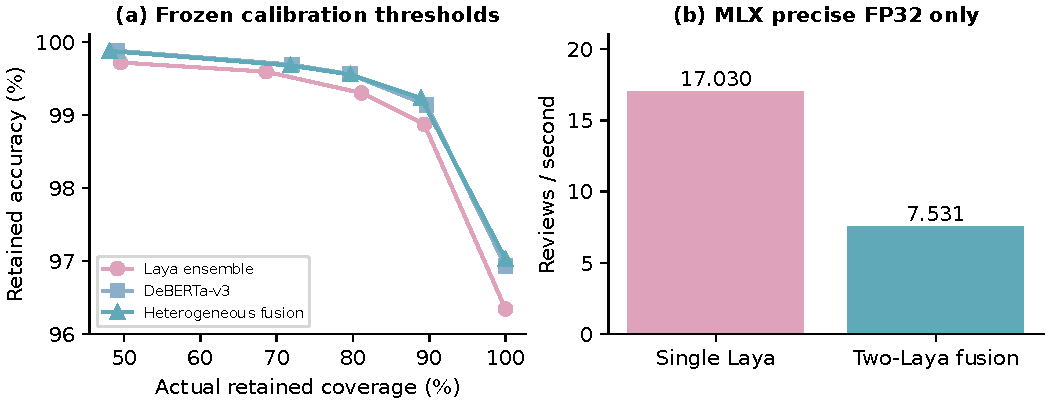
\includegraphics[width=\linewidth]{figures/09_selective_cost.pdf}\caption{左：以校准集冻结阈值获得的测试实际覆盖率与保留样本准确率；阈值未在测试上重新选择。右：此前的 MLX 精确 FP32 测量，仅比较单 Laya 与两个 Laya 的融合，作为最终三 checkpoint 系统的成本参照。}\label{fig:f10}\end{figure}
% Evidence: cases
\begin{table}[htbp]\centering\caption{开发集刻意选取的错误案例（原标签保持不变）}\label{tab:t6}\small\renewcommand{\arraystretch}{1.25}
\begin{tabularx}{\linewidth}{YYYY}\toprule
\textbf{样本 ID（train/ 后）} & \textbf{原标签} & \textbf{融合 p(pos)} & \textbf{定性解释}\\\midrule
neg/10566\_3.txt & 负 & 0.6833 & 同系列其他影片的好评干扰了对本片的判断\\
neg/11233\_2.txt & 负 & 0.9834 & 以低价为参照的挖苦，夹杂有限认可\\
pos/12230\_9.txt & 正 & 0.0580 & 制作较差但观看体验愉快\\
pos/3160\_7.txt & 正 & 0.0054 & 正文自评分与标签冲突（待核实）\\
\bottomrule\end{tabularx}\end{table}
% Evidence: cases;devanalysis
这些案例取自 47 条开发样本：此前的 Laya 主融合、2,048 上下文方案与 DeBERTa 在这 47 条上同时判错；它们不等于最终融合全部 68 条开发错误的集合。47 条中有 43 条在 Laya 与 DeBERTa 两种分词器下都未被截断，因此不能把所有共同错误都归因于上下文不足。模型判断一致也不意味着标签一定正确：评价对象、讽刺语气、观看乐趣与制作质量之间的错位，都可能造成语义误判。

% Evidence: cases
案例经过有目的选择，用于解释可能的失败方式；没有第二位标注者盲审，也没有据此估计总体错标率。正文—标签冲突仅标记待核实的数据问题，不作为修改开发标签、扣减错误或推断模型能力上限的依据。

\subsection{完整重训重复与权重探索}
% Evidence: supplement;suppprotocol
为考察模型组合变化的影响，在固定的 22,100 条梯度训练、400 条校准与 2,500 条开发划分上，预先固定三组种子：按 baseline、combined 与 DeBERTa 的顺序分别为（43,42,42）、（143,142,142）、（243,242,242）。九个模型均训练两轮并使用第二轮权重，经独立重载与校准后统一冻结，再在开发集上评价。全部重训在单张 RTX 4090 上完成；Laya 采用 FP32 训练，DeBERTa 采用 BF16 计算与 FP32 主参数；外层融合权重固定为 50:50。三个重复共享开发样本，不能视为 7,500 条独立记录。

% Evidence: supplement;suppweights
\begin{table}[htbp]\centering\caption{三组完整重训与事后权重探索的开发 Accuracy}\label{tab:t7}\small\renewcommand{\arraystretch}{1.25}
\begin{tabularx}{\linewidth}{YYYYY}\toprule
\textbf{方案} & \textbf{第一组} & \textbf{第二组} & \textbf{第三组} & \textbf{均值}\\\midrule
DeBERTa & 97.00\% & 97.28\% & 96.96\% & 97.080\%\\
等权融合 & 97.08\% & 97.36\% & 96.80\% & 97.080\%\\
DeBERTa 80\% & 97.04\% & 97.32\% & 97.04\% & 97.133\%\\
校准拟合权重 & 97.04\% & 97.36\% & 97.04\% & 97.147\%\\
\bottomrule\end{tabularx}\end{table}
% Evidence: supplement
等权融合在前两组各净多正确 2 条，在第三组净少正确 4 条，说明互补收益会随训练组合变化。三组平均 NLL 由 DeBERTa 的 0.091995 降至融合的 0.089649，平均 ECE 由 1.328\% 降至 0.741\%；三组 ECE 均低于 DeBERTa。与正确数的组间波动相比，ECE 的改善方向在三组中更一致。

% Evidence: suppweights
在上述重复完成后，另外固定加入 DeBERTa 权重为 80\% 的保守组合，以及仅在原 400 条校准数据上最小化 NLL 的单系数对照；模型温度及 Laya 内部系数沿用冻结值，所有候选和重复均保留。三组拟合得到的 DeBERTa 权重依次为 94.984\%、87.278\%、69.267\%，未使用开发标签选权重。80:20 方案相对 DeBERTa 分别净多正确 1、1、2 条；校准拟合方案分别净多正确 1、2、2 条。这些结果提示，降低较弱分支的权重是获得小幅增益的一个可行方向，值得在更多数据上继续验证。

% Evidence: supprobust
进一步按清洗文本组进行 10,000 次配对重采样，三组模型共享样本抽样；80:20 与校准拟合方案的平均准确率差条件 95\% 区间分别为 [−0.040, +0.160] 与 [−0.027, +0.160] 个百分点。区间在模型与后处理参数固定的条件下计算，不包含训练、参数拟合与研究选择的不确定性。

% Evidence: supprobust
在原 400 条校准数据上重复 10 次五折交叉验证，每折仅在训练部分重拟合温度、内部与外层权重。相对 DeBERTa，80:20 方案三组准确率均与 DeBERTa 持平，且 NLL 均更低；等权融合的三组平均留出 Accuracy 变化为 −0.325、−0.600、−0.100 个百分点；校准拟合方案的三组准确率变化为 0、0、−0.150 个百分点。该检查采用相同 NLL 目标与 [0.5,5] 温度范围，以基于逆温度凸性的二分法替代 Laya 历史实现中的 LBFGS 求解。300 次校准样本文本组重采样显示拟合权重会随样本组成变化，说明该权重应作为候选规则，而不是固定结论。因此，保守组合与概率质量改善呈现出值得继续研究的方向；候选规则的分类增益可在独立数据上进一步确认。

% Evidence: suppcases;suppweights
第三组等权融合相对 DeBERTa 修复 11 条错误、产生 15 条退化；15 条退化记录中，两个 Laya 模型均给出相同类别，13 条在两个 Laya 模型上的置信度都至少为 90\%，11 条在 Laya 下未被截断。提高 DeBERTa 权重在该组减少了退化，也会失去部分原有纠错：80:20 方案保留 2 次修复且没有新增退化。阅读这些案例可以看到褒贬混用、反讽，以及剧情情绪与作品评价相互交织的情况。上述观察说明平均概率在这些样本上如何越过 0.5 分类阈值，不构成对语义错误机制的因果解释。

\section{讨论、局限与可复现性}
\subsection{有效操作与创新边界}
% Evidence: final;supplement;suppweights;supprobust;suppcost
异构组合为当前 Laya 系统带来了明确的实测改进：在此前的固定方案上，官方测试净增 171 条正确，同时降低 NLL 与 ECE。相对 DeBERTa，原始的 50:50 组合及部分重训、权重配置呈现小幅准确率增益；不同配置下的收益幅度有所不同，为按场景选择融合权重提供了线索。三组重训中 ECE 改善方向一致，概率质量是本方案较稳定的收益来源。类型化决策头、DeBERTa、温度缩放与概率平均均为已有技术；本研究的价值在于将其适配到共同任务，并通过完整重复、误差变化与成本测量刻画适用条件。

\subsection{结果的适用范围}
% Evidence: final;audit;reviewaudit;supplement;suppweights;supprobust
官方测试、开发集及校准集曾用于历史研究，相关结果更适合作为固定方案在当前划分上的比较。实际梯度训练集与测试集有 113 条相同清洗文本，测试集内部还有 201 条额外重复记录；官方测试区间按类别分层构造，补充开发区间则按清洗文本组配对抽样。三组完整重训扩大了训练变化的观察范围，原官方测试仍对应一组固定权重；新增权重探索与交叉验证为后续确认提供了候选规则。因此，“部分配置观察到小幅提升”可理解为当前数据上的观察结果，其未来训练中的表现可在独立数据上进一步检验。

% Evidence: cpufull;suppcost
结果主要适用于二元、强极性的英语电影评论。完整开发集上的后端核验与同平台 GPU 测速补充了数值实现与计算代价证据；更大规模、混合批次以及不同运行后端的测速可用于进一步评估部署表现。对于极性更弱、其他语言或其他领域的数据，融合比例与校准效果需要重新评价。

\subsection{复现材料}
% Evidence: traincode;debertaconfig;final;suppprotocol;suppweights;supprobust
复现实验分为数据准备、模型训练、独立重载与校准、评估和融合诊断等步骤。每次运行都会保存数据划分、训练配置、锁定依赖、模型版本与逐样本预测；原固定评估、完整重训与事后权重检查分别归档，便于核对结果与追溯输入。

% Evidence: analysiscode
图表由冻结的摘要文件与逐样本预测生成，并据此复算正确数、混淆矩阵与概率指标。Scientific Agent Skills 用于辅助写作与图表审查\cite{skills}。

\subsection{已保留的逐轮训练记录}
% Evidence: curve
图~\ref{fig:f11} 展示历史 combined-s43 两轮训练中保存的平均训练损失与未校准开发准确率。该运行采用 seed 43，不是最终融合所用的 combined-s42；开发指标取自最终温度校准前的逐轮 checkpoint，不能代表最终方案结果。图中仅有两个逐轮观测点，连线用于识别顺序；本文不据此推断收敛过程，也不把训练 CE 与校准后的 NLL 当作同一种损失。

% Evidence: curve
\begin{figure}[htbp]\centering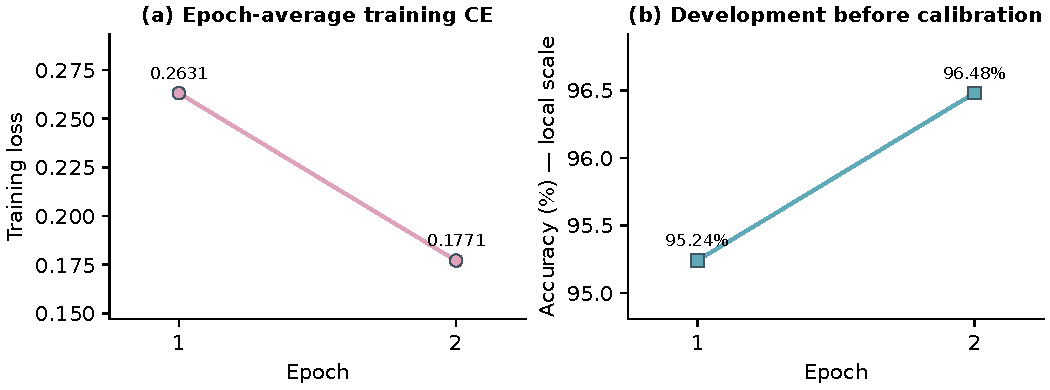
\includegraphics[width=\linewidth]{figures/10_training.pdf}\caption{历史 combined-s43 的逐轮训练损失与开发准确率。每轮开发分母为 2,500，指标未经最终温度校准；此运行不是最终融合成员。仅绘制已保存的两轮观测，没有补齐未保存的中间步骤。}\label{fig:f11}\end{figure}
\section{结论}
% Evidence: final;supplement;suppweights
本文构建并评估了多视图 Laya 与 DeBERTa-v3 的 IMDB 情感分类方案。完整官方测试上的结果为：Accuracy 97.028\%、Macro-F1 0.970280、NLL 0.092618、ECE 0.650\%；相对 Laya 双模型净多正确 171 条，相对 DeBERTa 净多正确 24 条，后者 McNemar p=0.1568。三组完整重训及权重探索进一步表明，该方案在部分配置中可以取得小幅准确率增益；三组等权融合的平均 Accuracy 与 DeBERTa 同为 97.08\%，平均 ECE 则从 1.328\% 降至 0.741\%。这些结果支持将误差互补与概率质量作为融合方案的主要评价维度，而不是预设每次组合都能提高分类正确数。

% Evidence: heads;robust;context;suppweights;supprobust;cpufull;suppcost
在本次开发记录上，保守权重与校准权重都带来小幅正向变化；完整的后处理五折交叉验证与配对区间进一步刻画了收益的配置与样本依赖，为后续确认实验提供了依据。考虑到三模型融合的推理开销，它更适合在重视概率质量、且计算预算允许的场景中继续研究。受控消融、跨后端核验与同平台测速共同提供了可复核的实验依据；后续重点是在独立数据上检验候选规则的可迁移性，并探索计算代价更低的组合方式。

\FloatBarrier\begin{thebibliography}{99}
\bibitem{maas} Maas A L, Daly R E, Pham P T, Huang D, Ng A Y, Potts C. Learning Word Vectors for Sentiment Analysis. ACL, 2011: 142–150. \url{https://aclanthology.org/P11-1015/}
\bibitem{modernbert} Warner B, Chaffin A, Clavié B, et al. Smarter, Better, Faster, Longer: A Modern Bidirectional Encoder for Fast, Memory Efficient, and Long Context Finetuning and Inference. arXiv:2412.13663, 2024. \url{https://arxiv.org/abs/2412.13663}
\bibitem{laya} Convai Innovations. Laya（英语模型）[模型]. Hugging Face. 访问日期：2026-10-19. \url{https://huggingface.co/convaiinnovations/laya}
\bibitem{deberta} He P, Gao J, Chen W. DeBERTaV3: Improving DeBERTa using ELECTRA-Style Pre-Training with Gradient-Disentangled Embedding Sharing. ICLR, 2023; arXiv:2111.09543. \url{https://arxiv.org/abs/2111.09543}
\bibitem{guo} Guo C, Pleiss G, Sun Y, Weinberger K Q. On Calibration of Modern Neural Networks. ICML, PMLR 70, 2017: 1321–1330. \url{https://proceedings.mlr.press/v70/guo17a.html}
\bibitem{wang} Wang S, Manning C. Baselines and Bigrams: Simple, Good Sentiment and Topic Classification. ACL (Volume 2: Short Papers), 2012: 90–94. \url{https://aclanthology.org/P12-2018/}
\bibitem{skills} Kassis T, Agarwal V, He Y, Patel D, Brueckner A M. Scientific Agent Skills: A Library of Procedural Knowledge for Research Agents. arXiv:2609.00065, 2026. \url{https://doi.org/10.48550/arXiv.2609.00065}
\bibitem{gce} Zhang Z, Sabuncu M R. Generalized Cross Entropy Loss for Training Deep Neural Networks with Noisy Labels. Advances in Neural Information Processing Systems 31, 2018. \url{https://papers.nips.cc/paper/2018/hash/f2925f97bc13ad2852a7a551802feea0-Abstract.html}
\end{thebibliography}\end{document}
